\documentclass{book}
\usepackage[papersize={204mm,275mm}, top=17mm,
bottom=17mm, outer=22mm, inner=20mm, includeheadfoot=false]{geometry}
\usepackage{lipsum}
\usepackage{commedit}
\clearpage
\begin{commeditPreamble}{commented.tex}
  \documentclass{book}
  \usepackage[papersize={230mm,288mm}, top=15mm,
  bottom=17mm, outer=11mm, inner=4.5mm, includeheadfoot=false]{geometry}
  \usepackage{kantlipsum}
  \usepackage{ragged2e}
  \usepackage{booktabs}
  \usepackage{commedit}
  \basepageargs{width=140mm}
  \commentsHook{\RaggedRight\parskip=0pt\parindent=1em\relax}
\end{commeditPreamble}

\begin{commeditText}
  \frontmatter
  \title{Commented edition}
  \author{Boris Veytsman}
  \date{November 2018}
  \maketitle
  
  \chapter{Introduction}
  \label{sec:intro-commented}

  This is the introuduction for the commented edition.  Note that we
  use \textsl{lipsum} for the base edition and \textsl{kantlipsum} for
  the commented edition.

  Some gibberish\footnote{We can use footnotes here.}\ldots
  
  \kant[6-20]

  \mainmatter

  \chapter{First chapter}
  \label{sec:first-commented}
\end{commeditText}

\begin{document}
\frontmatter
\title{Base edition}
\author{Boris Veytsman}
\date{November 2018}
\maketitle

\chapter{Foreword}
\label{chap:foreword}

The foreword for the base edition

\lipsum[1-5]

\begin{commeditText}

  Now we switch back to the commented edition\footnote{A footnote}.
  
  Some equation in the text.
  \begin{equation}
    \label{eq:pi}
    e^{i\pi}=-1,
  \end{equation}
  and another one
  \begin{equation}
    \label{eq:sin}
    sin^2\phi+\cos^2\phi=1.
  \end{equation}

  And more gibberish:

  \kant[5-12]
  
\end{commeditText}

\mainmatter

\chapter{Some thoughts}
\label{chap:thoughts}

Here we switch back to the base edition.  
\begin{commeditComments}
  Comments for the chapter~\ref{chap:thoughts} of the base
  edition\footnote{A footnote}.
  \begin{equation}
    e=mc^2
  \end{equation}
  \kant[6]
\end{commeditComments}

An equation for the base edition:
\begin{equation}
  \label{eq:Einstein}
  e=mc^2.
\end{equation}

And pseudo-lating gibberish.

\lipsum[6-12]


\begin{commeditComments}
  We can reference base equation~(\ref{eq:Einstein}) on base
  page~(\pageref{eq:Einstein}) and commented edition
  equations~(\ref{eq:pi}) and (\ref{eq:sin}) on the commented edition
  page~(\pageref{eq:pi}).

  More gibberish\footnote{A footnote for the comments.}.
  
  \kant[7]
\end{commeditComments}

More gibberish for base edition.

\lipsum[15-17]

\begin{commeditComments}
  Comments.
  \kant[4]
  \begin{equation}
    u=v\cdot a
  \end{equation}
\end{commeditComments}

\lipsum[3-2]

\begin{commeditComments}
  \begin{itemize}
  \item item
  \item item
  \item item
  \end{itemize}

  
  \pagebreak
  More comments.  Note the continuation pages\ldots
  \kant[8-20]
\end{commeditComments}

\lipsum[9-20]

\begin{commeditComments}
  Here we add a figure.

  \begin{figure}
    \centering
    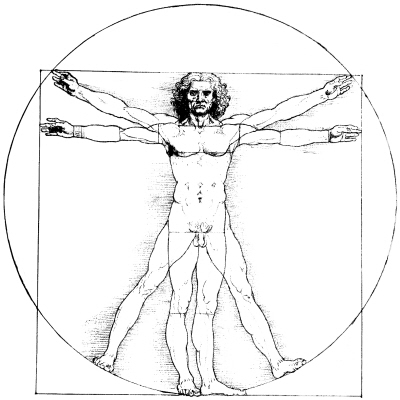
\includegraphics[width=\columnwidth]{vitruvian}
    \caption{Vitruvian man}
    \label{fig:vitruvian}
  \end{figure}

  There is no difference between starred and unstarred floats
  \begin{table*}
    \centering
    \begin{tabular}{ll}
      \toprule
      Gnus & Gnats\\
      \midrule
      12 & 20\\
      24 & 10\\
      \bottomrule
    \end{tabular}
    \caption{A table}
    \label{tab:table}
  \end{table*}

\end{commeditComments}

\begin{commeditText}
  \section{Final text}


  Here we add a real float.  Note that it floats to the top of the
  page.

  \begin{figure}[t]
    \centering
    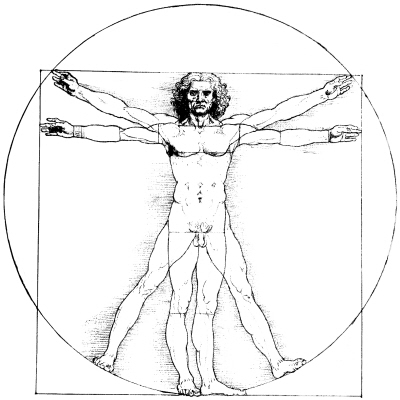
\includegraphics[width=.5\columnwidth]{vitruvian}    
    \caption{Another vitruvian man}
    \label{fig:vitruvian1}
  \end{figure}
\end{commeditText}

\end{document}
